\section*{Aufgabe 2}
\subsection*{a)}
Denken Sie sich eine kleine Sprache aus.
Definieren Sie deren Vokabular mit einer ANTLR4 lexer grammar und deren Grammatik mit einer ANTLR4 parser grammar.
Erzeugen Sie für einige Beispieltexte mit Hilfe von \textit{org.antlr.v4.gui.TestRig} den Ableitungsbaum (Parse Tree).

\subsection*{a - Lösung}
Dargestellt ist der Lexer einer Sprache, welche die Klammerung von Ausdrücken überprüft.
Erlaubt sind Variablen - also einzelne Buchstaben, sowie Zahlen.
Konkateniert werden Ausdrücke mit den Operatoren: \texttt{+}, \texttt{-}, \texttt{*}, \texttt{/}.
\newline
\begin{lstlisting}[label={lst:Aufgabe2a_lexer}, style=ANTLR]
    // ParenthesesLexer.g4
    lexer grammar ParenthesesLexer;

    ROUND_OPEN : '(';
    ROUND_CLOSE : ')';
    SQUARE_OPEN : '[';
    SQUARE_CLOSE : ']';
    CURLY_OPEN : '{';
    CURLY_CLOSE : '}';

    VARIABLE : [a-z];

    NUMBER : [1-9][0-9]*;

    OPERATOR: [+\-*/];

    WS : [ \t\r\n]+ -> skip;
\end{lstlisting}

\newpage

Der dazugehörige Parser:
\begin{lstlisting}[label={lst:Aufgabe2a_parser}, style=ANTLR]
    // ParenthesesParser.g4
    parser grammar ParenthesesParser;
    options { tokenVocab=ParenthesesLexer; }

    expr: expr OPERATOR expr | roundExpr | squareExpr | curlyExpr | atom;

    roundExpr: ROUND_OPEN expr ROUND_CLOSE;
    squareExpr: SQUARE_OPEN expr SQUARE_CLOSE;
    curlyExpr: CURLY_OPEN expr CURLY_CLOSE;

    atom: VARIABLE | NUMBER;
\end{lstlisting}
\newline

\begin{figure}[h]
    \centering
    \subfloat[\centering Input: (1 + b)]{{ 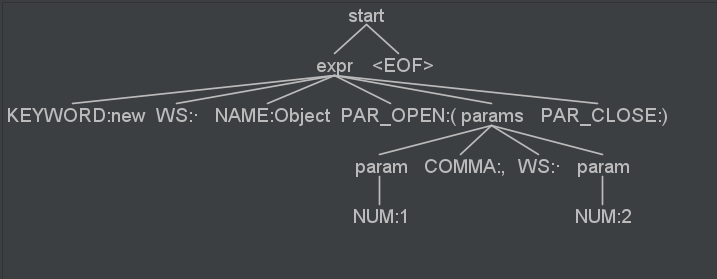
\includegraphics[width=5cm]{images/Aufgabe2a_parseTree_simple} }}
    \qquad
    \subfloat[\centering Input: (14 / a + 2)]{{ 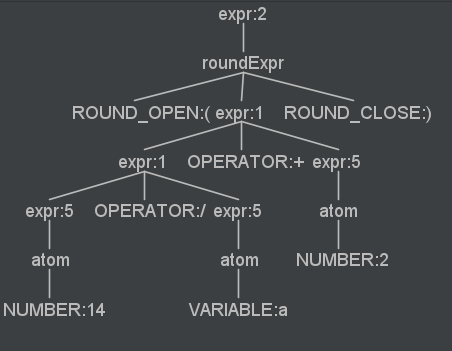
\includegraphics[width=5cm]{images/Aufgabe2a_parseTree} }}
    \caption{Parse Tree Beispiele}
    \label{fig:Aufgabe2a_parseTree}
\end{figure}
\newline

\textbf{Der Parser ist für die grammatikalische Anordnung der durch den Lexer vorgegebenen Token verantwortlich.}
\newpage